For both experiments, 15$\%$ of the data was held out as a test and validation set each. The  exact breakdowns of the sets can be seen in Appendix .Recall was utilized to measure performance ($\%$ of true positives in top 10 and 1000 of predictions). Gridsearchs were used to run models with all posible combinations of chosen configurations. The models were also evaluated with early-stopping (training was stopped when model exhibited maximum performance on the validation set) to prevent over-fitting.

\subsection{Experimental Setup: RankFromSets}
\acrshort{rfs} was run using RMSProp optimizer~\parencite{tieleman2012lecture} with a momentum of 0.9 and a gridsearch was done over learning rates of $\{10^{-2}, 10^{-3}, 10^{-4}, 10^{-5}\}$, embedding sizes of $\{10, 25, 50, 100, 500, 1000\}$, and a decision of whether or not to pre-initialize the model with BERT embeddings. The basic training loop is shown here:
\begin{minted}{python}
for step, batch in enumerate(cycle(train_loader)):
    # turn to training mode and calculate loss for backpropagation
    torch.enable_grad()
    model.train()
    optimizer.zero_grad()
    publications, articles, word_attributes, attribute_offsets, real_labels = batch
    publication_set = [args.target_publication] * len(real_labels)
    publication_set = torch.tensor(publication_set, dtype=torch.long)
    publication_set = publication_set.to(device)
    articles = articles.to(device)
    word_attributes = word_attributes.to(device)
    attribute_offsets = attribute_offsets.to(device)
    logits = model(publication_set, articles, word_attributes, attribute_offsets)
    L = loss(logits, labels)
    L.backward()
    optimizer.step()
    running_loss += L.item()
\end{minted}

\subsection{Experimental Setup: BERT}
As \acrshort{bert} already comes "pre-trained", I fine-tuned it to the collected data with the AdamW optimizer and a linear learning rate scheduler with warm up steps according to best practices, as outlined by ~\textcite{devlin2019bert:} and ~\textcite{wolf2019huggingfaces}. The model used a batch size of 32, and articles had maximum length of 512 tokens. A grid search was performed over learning rates of $\{2, 3, 4, 5\} \times 10^{-5}$, warmup steps of $\{10^2, 10^3, 10^4\}$, and total training steps $\{10^2, 10^3, 10^4, 10^5\} \times 5$. The basic training loop is shown here:
\begin{minted}{python}
for step, batch in enumerate(cycle(train_loader)):
    # turn to training mode and calculate loss for backpropagation
    torch.enable_grad()
    optimizer.zero_grad()
    word_attributes, attention_masks, word_subset_counts, real_labels = batch
    word_attributes = word_attributes.to(device)
    attention_masks = attention_masks.to(device)
    logits = model(word_attributes, attention_masks)[0]
    logits = torch.squeeze(logits)
    L = loss(logits, labels)
    L.backward()
    if args.clip_grad:
        nn.utils.clip_grad_norm_(model.parameters(), 1.0)
    optimizer.step()
    scheduler.step()
    running_loss += L{}.item()
\end{minted}

\subsection{Quantitative Evaluation}
The best performing models from both approaches were chosen, and were evaluated via recall on the test set.
% !TEX root = ../proceedings.tex
\begin{table}[h]
\centering
\begin{tabular}{lSS}
\toprule
Recommendation Model & \multicolumn{1}{c}{Recall @ 1000 (\%)}
\\
\midrule
\acrlong{rfs} &  \bfseries 53.1\\
\acrshort{bert} & 46.6 \\
\bottomrule
\end{tabular}
% BERT 466/1000
% rankfromsets 531/1000
% \vspace{1ex}
\caption{\gls{rfs} outperforms \acrshort{bert} in an offline evaluation on the test dataset when predicting which articles would be featured at The Browser}
\label{tab:recall}
\end{table}

Additionally, the time taken to train the models is shown:

% !TEX root = ../recommending-interesting-writing.tex
\begin{figure}[h]
  \centering
  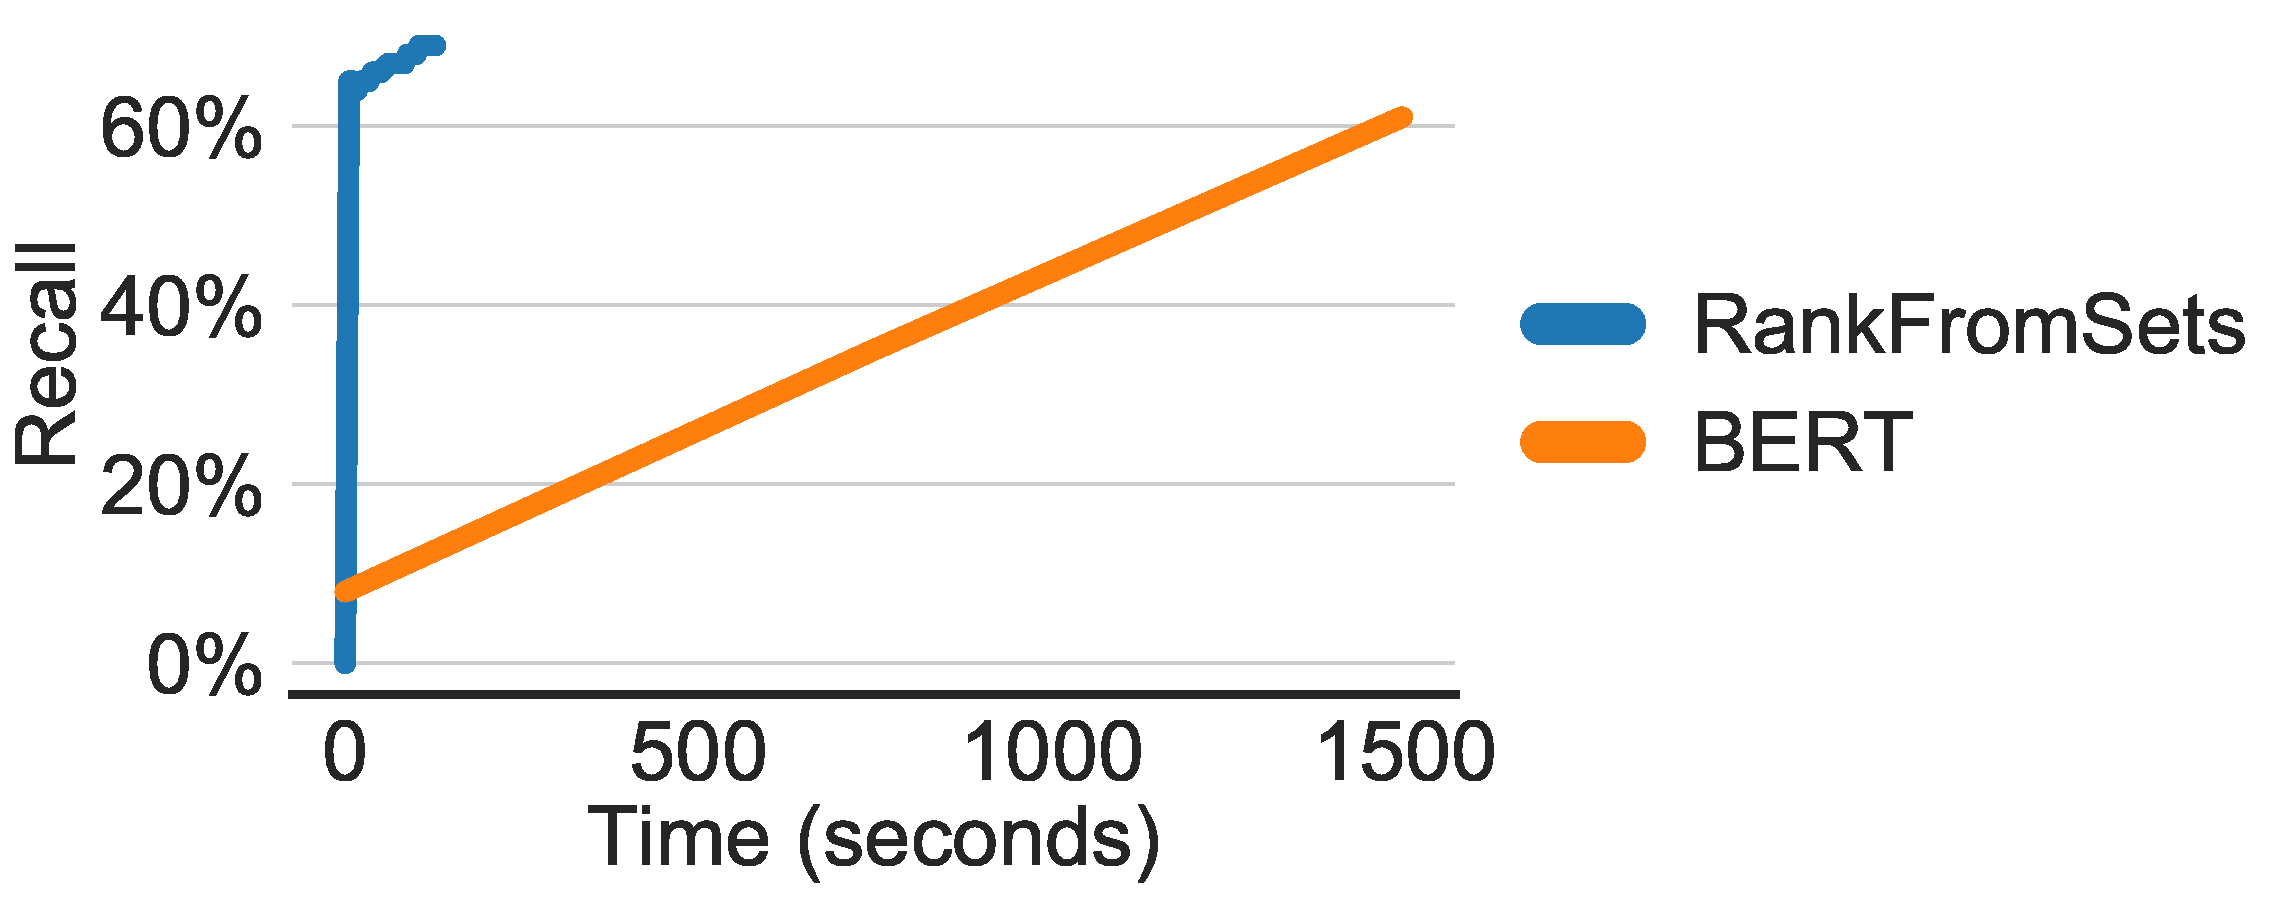
\includegraphics[width=0.95\linewidth]{fig/training-recall}
  \caption{\acrshort{rfs} achieves better performance faster than \acrshort{bert} in terms of validation recall during training.}
  \label{fig:training-recall}
\end{figure}